\documentclass{standalone}
\usepackage{tikz}
%------------tikz Setup------------

\tikzstyle{ball} = [circle,shading=ball, ball color=black,
    minimum size=1mm,inner sep=1.3pt]
\tikzstyle{miniball} = [circle,shading=ball, ball color=black,
    minimum size=1mm,inner sep=0.5pt]
\tikzstyle{mminiball} = [circle,shading=ball, ball color=black,
    minimum size=0.6mm,inner sep=0.1pt]
\usetikzlibrary{arrows.meta}
\usetikzlibrary{angles, quotes}
\tikzset{>={Latex[length=2mm,width=1.5mm]}}
\tikzset{->-/.style={decoration={markings, mark=at position #1 with
  {\arrow{>}}},postaction={decorate}}}
\usetikzlibrary{decorations.pathmorphing}
\usetikzlibrary{decorations.pathreplacing}
\usetikzlibrary{arrows.meta,calc}
\usetikzlibrary{bending}
\usetikzlibrary{decorations.markings,shapes.geometric}
\tikzset{->-/.style={decoration={markings, mark=at position #1 with
  {\arrow{>}}},postaction={decorate}}}
\tikzset{-|-/.style={decoration={markings, mark=at position #1 with
  {\arrow{stealth}}},postaction={decorate}}}
\tikzset{movearrow/.style 2 args ={
        decoration={markings,
    mark= at position {#1} with {\arrow{#2}} ,
        },
        postaction={decorate}
    }
}


\begin{document}
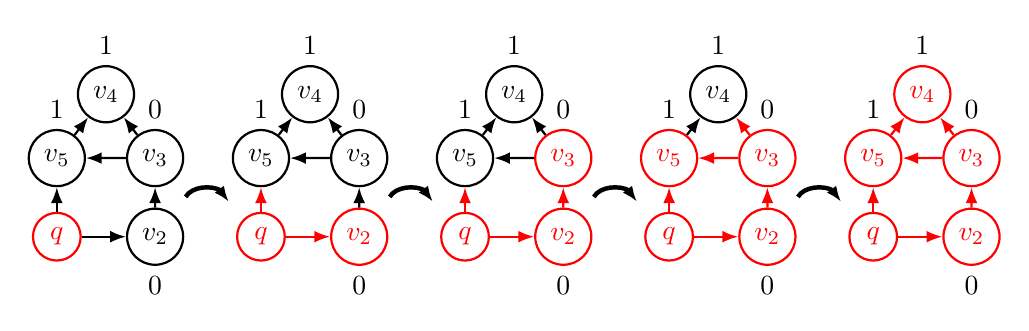
\begin{tikzpicture}[thick,main/.style = {draw, circle},scale=0.96]
\begin{scope}[scale=0.65]
    \node[main,red] (1) at (0,0) {$q$}; 
    \node[main,label={below:$0$}] (2) at (2,0) {$v_2$}; 
    \node[main,label={above:$0$}] (3) at (2,1.6) {$v_3$};
    \node[main,label={above:$1$}] (4) at (1,2.9) {$v_4$};
    \node[main,label={above:$1$}] (5) at (0,1.6) {$v_5$};
    \draw[thick,->] (1) to (2);
    \draw[thick,->] (1) to (5);
    \draw[thick,->] (2) to (3);
    \draw[thick,->] (3) to (5);
    \draw[thick,->] (3) to (4);
    \draw[thick,->] (5) to (4);
    \node (a) at (2.5, 0.6) {};
    \node (b) at (3.5, 0.5) {};
    \draw[ultra thick,->] (a) to [out=60,in=90] (b);
\end{scope}
\begin{scope}[xshift=2.7cm,scale=0.65]
    \node[main,red] (1) at (0,0) {$q$}; 
    \node[main,red,label={below:$0$}] (2) at (2,0) {$v_2$}; 
    \node[main,label={above:$0$}] (3) at (2,1.6) {$v_3$};
    \node[main,label={above:$1$}] (4) at (1,2.9) {$v_4$};
    \node[main,label={above:$1$}] (5) at (0,1.6) {$v_5$};
    \draw[thick,->,red] (1) to (2);
    \draw[thick,->,red] (1) to (5);
    \draw[thick,->] (2) to (3);
    \draw[thick,->] (3) to (5);
    \draw[thick,->] (3) to (4);
    \draw[thick,->] (5) to (4);
    \node (a) at (2.5, 0.6) {};
    \node (b) at (3.5, 0.5) {};
    \draw[ultra thick,->] (a) to [out=60,in=90] (b);
\end{scope}
\begin{scope}[xshift=5.4cm,scale=0.65]
    \node[main,red] (1) at (0,0) {$q$}; 
    \node[main,red,label={below:$0$}] (2) at (2,0) {$v_2$}; 
    \node[main,red,label={above:$0$}] (3) at (2,1.6) {$v_3$};
    \node[main,label={above:$1$}] (4) at (1,2.9) {$v_4$};
    \node[main,label={above:$1$}] (5) at (0,1.6) {$v_5$};
    \draw[thick,->,red] (1) to (2);
    \draw[thick,->,red] (1) to (5);
    \draw[thick,->,red] (2) to (3);
    \draw[thick,->] (3) to (5);
    \draw[thick,->] (3) to (4);
    \draw[thick,->] (5) to (4);
    \node (a) at (2.5, 0.6) {};
    \node (b) at (3.5, 0.5) {};
    \draw[ultra thick,->] (a) to [out=60,in=90] (b);
\end{scope}
\begin{scope}[xshift=8.1cm,scale=0.65]
    \node[main,red] (1) at (0,0) {$q$}; 
    \node[main,red,label={below:$0$}] (2) at (2,0) {$v_2$}; 
    \node[main,red,label={above:$0$}] (3) at (2,1.6) {$v_3$};
    \node[main,label={above:$1$}] (4) at (1,2.9) {$v_4$};
    \node[main,red,label={above:$1$}] (5) at (0,1.6) {$v_5$};
    \draw[thick,->,red] (1) to (2);
    \draw[thick,->,red] (1) to (5);
    \draw[thick,->,red] (2) to (3);
    \draw[thick,->,red] (3) to (5);
    \draw[thick,->,red] (3) to (4);
    \draw[thick,->] (5) to (4);
    \node (a) at (2.5, 0.6) {};
    \node (b) at (3.5, 0.5) {};
    \draw[ultra thick,->] (a) to [out=60,in=90] (b);
\end{scope}
\begin{scope}[xshift=10.8cm,scale=0.65]
    \node[main,red] (1) at (0,0) {$q$}; 
    \node[main,red,label={below:$0$}] (2) at (2,0) {$v_2$}; 
    \node[main,red,label={above:$0$}] (3) at (2,1.6) {$v_3$};
    \node[main,red,label={above:$1$}] (4) at (1,2.9) {$v_4$};
    \node[main,red,label={above:$1$}] (5) at (0,1.6) {$v_5$};
    \draw[thick,->,red] (1) to (2);
    \draw[thick,->,red] (1) to (5);
    \draw[thick,->,red] (2) to (3);
    \draw[thick,->,red] (3) to (5);
    \draw[thick,->,red] (3) to (4);
    \draw[thick,->,red] (5) to (4);
\end{scope}
\end{tikzpicture}
\end{document}